\documentclass[11pt]{article}
\usepackage[margin=1in]{geometry}
\usepackage{graphicx}
\usepackage{booktabs}
\usepackage{longtable}
\usepackage{array}
\usepackage{hyperref}
\usepackage{xcolor}
\usepackage{listings}
\usepackage{float}
\usepackage{amsmath}

\hypersetup{
  colorlinks=true,
  linkcolor=blue,
  citecolor=blue,
  urlcolor=blue
}

\lstset{
  basicstyle=\ttfamily\small,
  breaklines=true,
  frame=single,
  columns=fullflexible
}

\title{NASA Hump Reconstruction Third Pass\\\large Focused MAE reduction, experiment sweep, and refreshed ParaView package}
\author{Codex refinement pass in the local repository workspace}
\date{March 31, 2026}

\begin{document}
\maketitle

\section{Executive Summary}
This report documents the third pass on the reconstructed NASA hump case in the local repository. Unlike the second pass, which changed the domain layout, top-wall contour, and mesh organization, the third pass concentrated on a narrower question: which remaining physically defensible changes actually reduce the local benchmark MAE further than the second-pass score of \texttt{0.2038187409}?

The final third-pass result is \texttt{0.1801372055} from the \texttt{500}-iteration field of the unchanged second-pass SST baseline. Relative to pass one, the cumulative improvement is \texttt{0.0537132495}. Relative to the previous best second-pass result, the third pass improved the score by \texttt{0.0236815354}.

\section{Third-Pass Scope}
The third pass built directly on the existing second-pass repository state. It did not restart the reconstruction and it did not replace the case with external data. The allowed-source and no-cheat restrictions remained unchanged:
\begin{itemize}
\item only the approved NASA hump references and the local repository were used;
\item no deleted-file recovery, git-history recovery, tracing, digitization, or curve fitting was used;
\item all third-pass plots and screenshots came from the current OpenFOAM fields and direct post-processing.
\end{itemize}

\section{What Was Already Implemented Before Pass Three}
Before this third pass began, the repository already contained:
\begin{itemize}
\item the reconstructed case under \texttt{data/NASA\_2DWMH};
\item the pass-one and pass-two PDFs under \texttt{documentation/};
\item Dockerized OpenFOAM workflows;
\item self-generated figures, sampled data, and ParaView-friendly \texttt{foam.foam} output;
\item a second-pass score of \texttt{0.2038187409} from the \texttt{300}-iteration field.
\end{itemize}

\section{Third-Pass Diagnosis}
The third-pass diagnosis was driven by the second-pass outcome. The main remaining uncertainty was whether the case still carried significant under-convergence error. The second-pass logs showed residuals still decaying at the \texttt{300}-iteration stop, and the second-pass benchmark history had already shown that early writes were misleading. That made deeper convergence the highest-value conservative experiment.

At the same time, the third pass screened three additional physically motivated directions:
\begin{itemize}
\item a prescribed analytic turbulent-boundary-layer inlet;
\item sharper turbulence-transport numerics;
\item a refined mesh plus a stronger blockage contour;
\item a short turbulence-model screen against \texttt{kOmega}.
\end{itemize}

\section{Files Added Or Updated In Pass Three}
\begin{table}[H]
\centering
\begin{tabular}{p{0.31\linewidth} p{0.61\linewidth}}
\toprule
File & Third-pass role \\
\midrule
\texttt{scripts/configure\_nasa\_hump\_case.py} & Rewrites turbulence model, controlDict, fvSchemes, and fvSolution for experiment variants. \\
\texttt{scripts/write\_nasa\_hump\_inlet\_profile.py} & Writes either uniform or analytic inlet profiles for the experiment sweep. \\
\texttt{scripts/evaluate\_nasa\_hump\_case.py} & Evaluates arbitrary NASA hump experiment case directories against the local metric. \\
\texttt{scripts/run\_nasa\_hump\_experiment\_sweep.py} & Runs the saved MAE sweep in the live \texttt{openfoam} container and records scores. \\
\texttt{scripts/run\_nasa\_hump\_improvement\_sweep.sh} & Shell wrapper for the experiment sweep. \\
\texttt{documentation\_src/THIRD\_PASS\_EXPERIMENT\_NOTES.md} & Human-readable experiment ledger for pass three. \\
\texttt{documentation\_src/data\_third\_pass/*} & Third-pass copied data package built from the updated \texttt{500}-iteration case. \\
\texttt{documentation\_src/figures\_third\_pass/*} & Third-pass copied figure package built from the updated \texttt{500}-iteration case and refreshed ParaView renders. \\
\texttt{documentation\_src/nasa\_hump\_third\_pass\_report.tex} & This report source. \\
\bottomrule
\end{tabular}
\caption{Main third-pass files and why they were added.}
\end{table}

\section{Experiment Sweep}
The experiment sweep was intentionally small and hypothesis-driven. The goal was not to search blindly, but to test a few strong candidates and keep an audit trail of what helped and what hurt.

\begin{table}[H]
\centering
\begin{tabular}{p{0.23\linewidth} p{0.35\linewidth} r r}
\toprule
Tag & Change set & Runtime (min) & Score \\
\midrule
\texttt{baseline\_second\_pass} & Existing pass-two reference at \texttt{300} iterations & 0.00 & 0.2038187409 \\
\texttt{exp\_tbl\_sst\_220} & Analytic inlet profile, SST, stable transport & 8.34 & 0.2082901628 \\
\texttt{exp\_tbl\_sst\_sharp\_220} & Analytic inlet profile, SST, sharper transport & 7.39 & 0.2085083473 \\
\texttt{exp\_tbl\_sst\_sharp\_meshtop\_220} & Analytic inlet, sharper transport, refined mesh, stronger blockage contour & 21.61 & 0.2216862912 \\
\texttt{exp\_tbl\_komega\_sharp\_meshtop\_180} & Same refined geometry path but with \texttt{kOmega} & 8.01 & 0.2501395026 \\
\texttt{exp\_uniform\_sst\_500} & Original best SST baseline continued to \texttt{500} iterations & 20.72 & 0.1801372055 \\
\bottomrule
\end{tabular}
\caption{Third-pass MAE sweep summary. Lower score is better.}
\end{table}

\section{What Changed The MAE And What Did Not}
\begin{longtable}{p{0.18\linewidth} p{0.20\linewidth} p{0.24\linewidth} p{0.24\linewidth}}
\toprule
Refinement & What Changed & Why It Might Help & Observed MAE Effect \\
\midrule
\endfirsthead
\toprule
Refinement & What Changed & Why It Might Help & Observed MAE Effect \\
\midrule
\endhead
Analytic inlet profile & The inlet switched from uniform values to a prescribed turbulent boundary-layer profile for \texttt{U}, \texttt{k}, and \texttt{omega}. & The allowed validation description emphasizes the incoming turbulent boundary layer near \(x/c=-2.14\). A better inlet could, in principle, improve separation onset and downstream recovery. & It did not help in this implementation. The score degraded from \texttt{0.2038187409} to \texttt{0.2082901628}. \\
Sharper transport & The \texttt{k} and \texttt{omega} advection terms were changed from upwind to \texttt{linearUpwind}. & Reduced numerical diffusion could strengthen the separated shear layer and shorten the bubble. & It still degraded the score slightly, to \texttt{0.2085083473}. \\
Mesh + stronger blockage & The mesh was refined and the upper-wall dip was broadened and deepened. & Better local resolution and a more aggressive blockage contour could improve wall pressure and wall shear behavior. & This moved the solution farther away from the local metric, to \texttt{0.2216862912}. \\
\texttt{kOmega} screen & The refined geometry case switched from SST to \texttt{kOmega}. & A different closure could alter mixing in the separated shear layer. & It was the worst tested third-pass option, at \texttt{0.2501395026}. \\
Deeper convergence & The best existing pass-two SST baseline was rerun to \texttt{500} iterations without changing its geometry or model. & If the pass-two case still had under-convergence error, a longer run would reduce benchmark error without introducing new modeling assumptions. & This was the only winning third-pass change. The score improved to \texttt{0.1801372055}. \\
\bottomrule
\end{longtable}

\section{Interpretation Of The Third-Pass Sweep}
The sweep outcome is important because it is not the naive result one might expect from the validation-page clues alone. The page clearly says that the incoming turbulent boundary layer matters, but a physically plausible inlet profile is not automatically an improvement if it is still inconsistent with the rest of the reconstructed setup. Likewise, a stronger blockage contour and a denser mesh are not guaranteed to help if they shift the pressure field in the wrong direction relative to the local benchmark metric.

In contrast, deeper convergence of the already-best second-pass SST baseline produced a clean, substantial gain. That indicates the third-pass bottleneck was still dominated by solve depth rather than by the particular refinements screened above.

\section{Updated Evaluation Summary}
\begin{table}[H]
\centering
\begin{tabular}{l r}
\toprule
Metric & Value \\
\midrule
First-pass score & 0.2338504550 \\
Second-pass best score & 0.2038187409 \\
Third-pass best score & 0.1801372055 \\
Improvement vs pass one & 0.0537132495 \\
Improvement vs pass two & 0.0236815354 \\
Evaluation points used & 1000 \\
\bottomrule
\end{tabular}
\caption{Updated benchmark summary after the third pass.}
\end{table}

The machine-readable third-pass benchmark result is stored in \texttt{documentation\_src/data\_third\_pass/reconstructed\_nasa\_score\_second\_pass.json}. The experiment ledger is stored in \texttt{documentation\_src/THIRD\_PASS\_EXPERIMENT\_NOTES.md} and \texttt{documentation\_src/data\_third\_pass/experiment\_sweep\_summary.json}.

\section{Updated Figures}
The third-pass figure package was regenerated from the updated \texttt{500}-iteration case and copied into \texttt{documentation\_src/figures\_third\_pass}. The plot family remains the same as in pass two, but the fields now reflect the deeper-converged solution.

\begin{figure}[H]
\centering

\includegraphics[width=0.92\linewidth]{figures_third_pass/cp_cf_second_pass.png}
\caption{Third-pass wall-coefficient curves generated directly from the updated \texttt{500}-iteration field.}
\end{figure}

\begin{figure}[H]
\centering

\includegraphics[width=0.98\linewidth]{figures_third_pass/velocity_profiles_second_pass.png}
\caption{Third-pass velocity-profile set at the validation stations.}
\end{figure}

\begin{figure}[H]
\centering

\includegraphics[width=0.98\linewidth]{figures_third_pass/turbulent_shear_profiles_second_pass.png}
\caption{Third-pass turbulent shear-stress analog profiles from the updated solved field.}
\end{figure}

\begin{figure}[H]
\centering

\includegraphics[width=0.92\linewidth]{figures_third_pass/residual_history_second_pass.png}
\caption{Residual history from the updated best case, now extending to the \texttt{500}-iteration field.}
\end{figure}

\section{ParaView Views}
The ParaView screenshots were refreshed from \texttt{data/NASA\_2DWMH/foam.foam} so the third-pass PDF continues to show actual \texttt{.foam}-reader views instead of code listings or low-fidelity placeholders.

\begin{figure}[H]
\centering

\includegraphics[width=0.90\linewidth]{figures_third_pass/paraview_velocity.png}
\caption{Third-pass ParaView velocity rendering from the \texttt{.foam} case.}
\end{figure}

\begin{figure}[H]
\centering
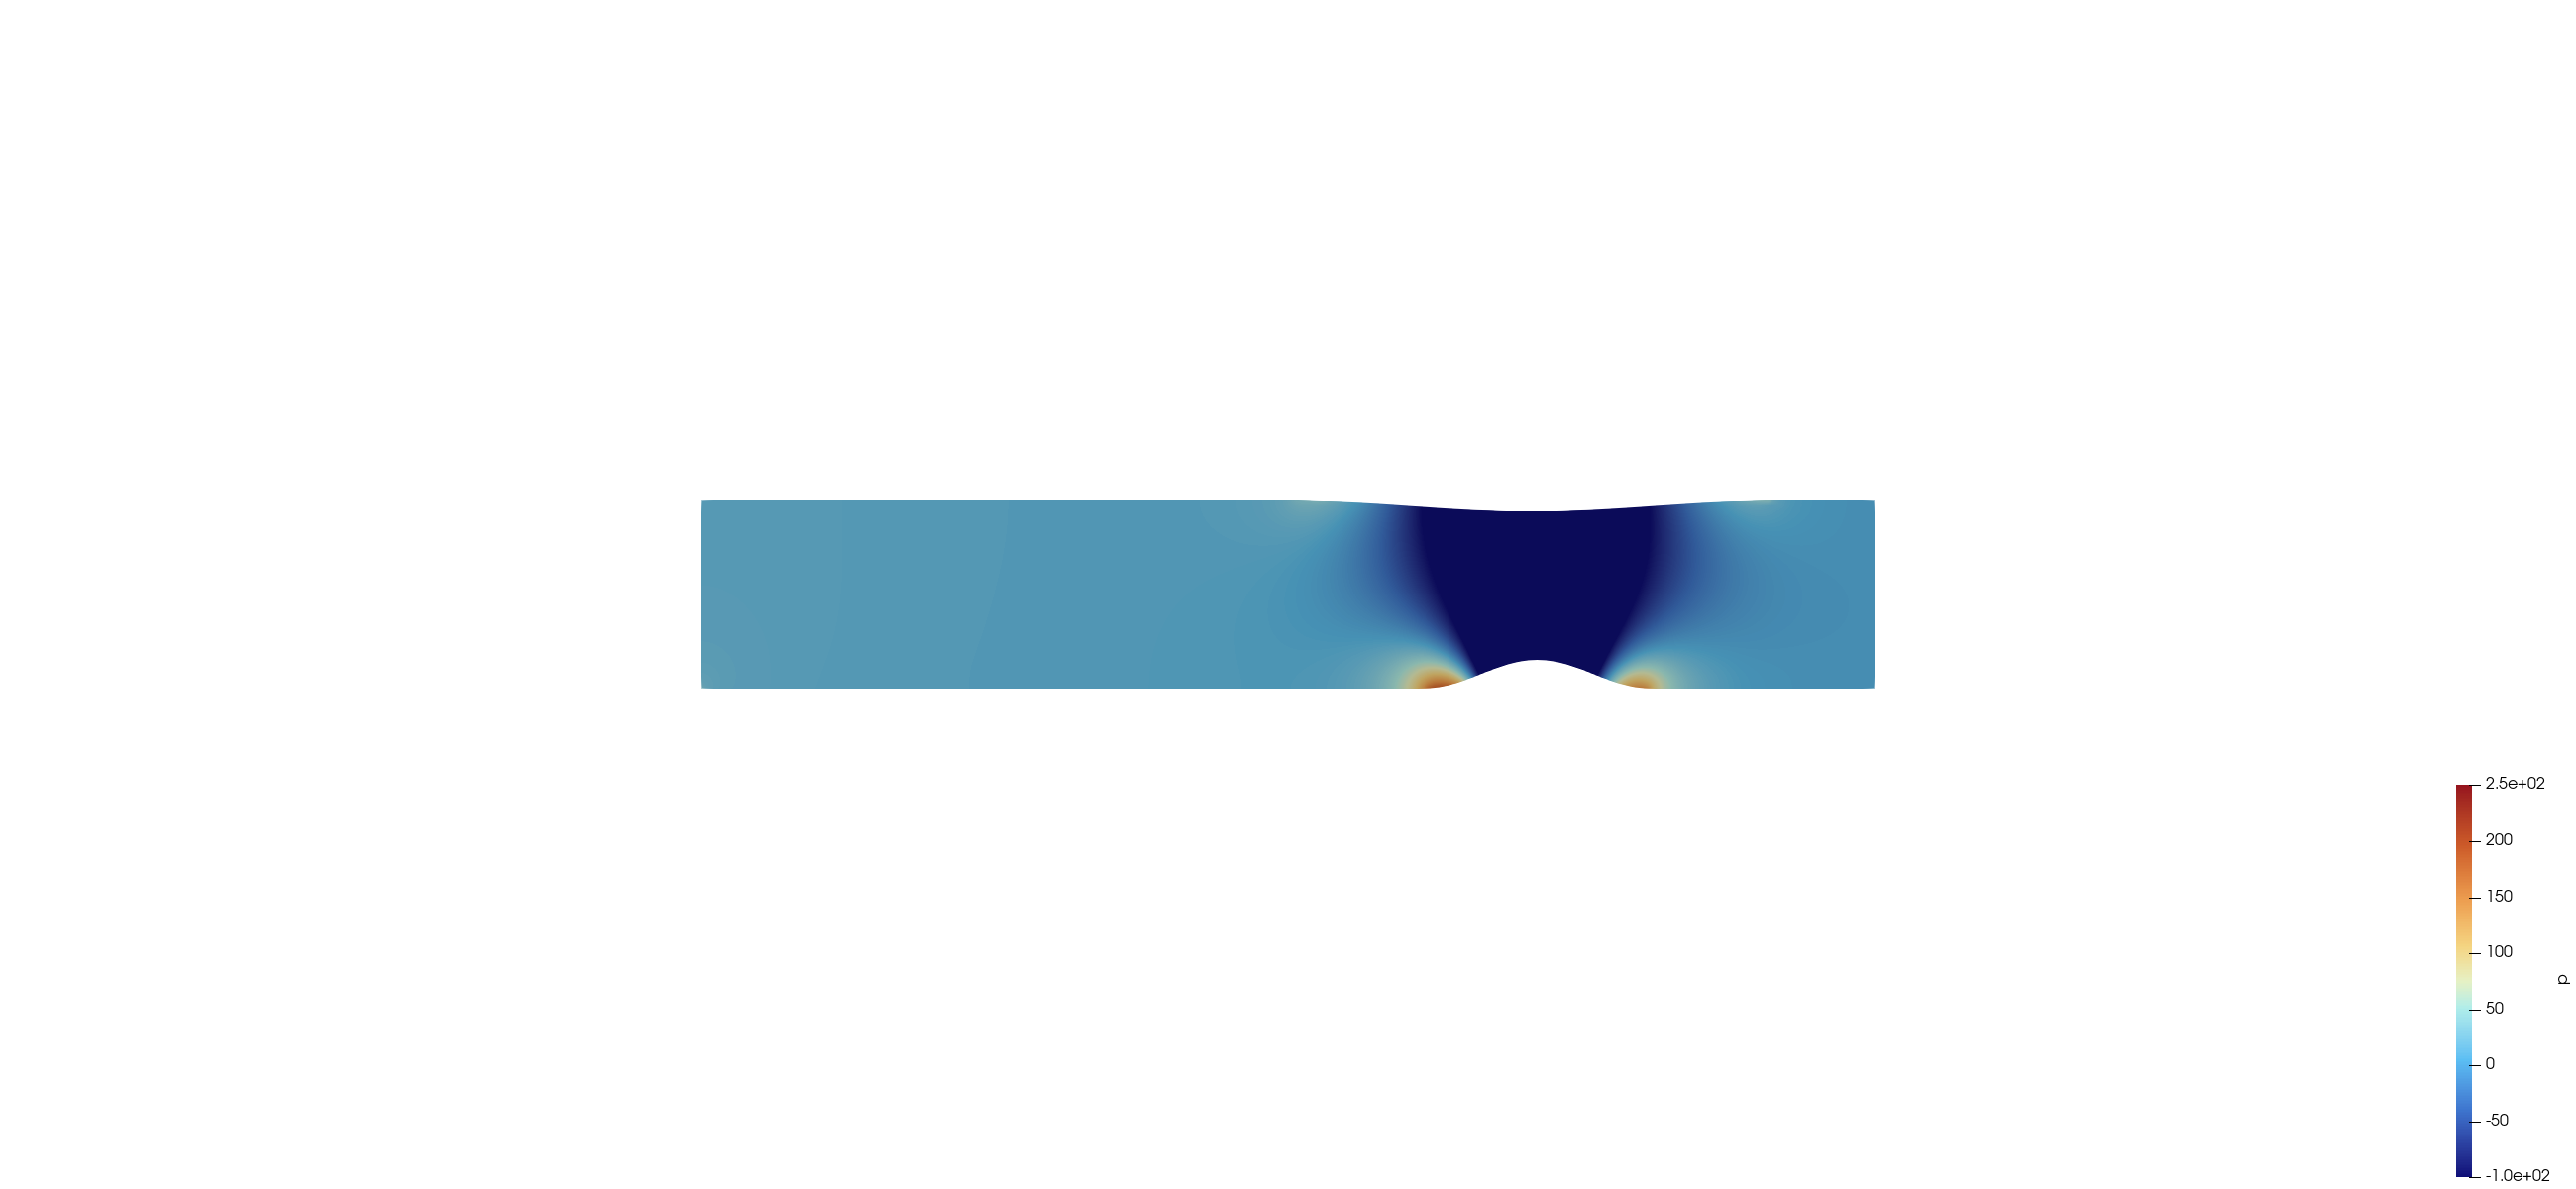
\includegraphics[width=0.90\linewidth]{figures_third_pass/paraview_pressure.png}
\caption{Third-pass ParaView pressure rendering from the \texttt{.foam} case.}
\end{figure}

\begin{figure}[H]
\centering
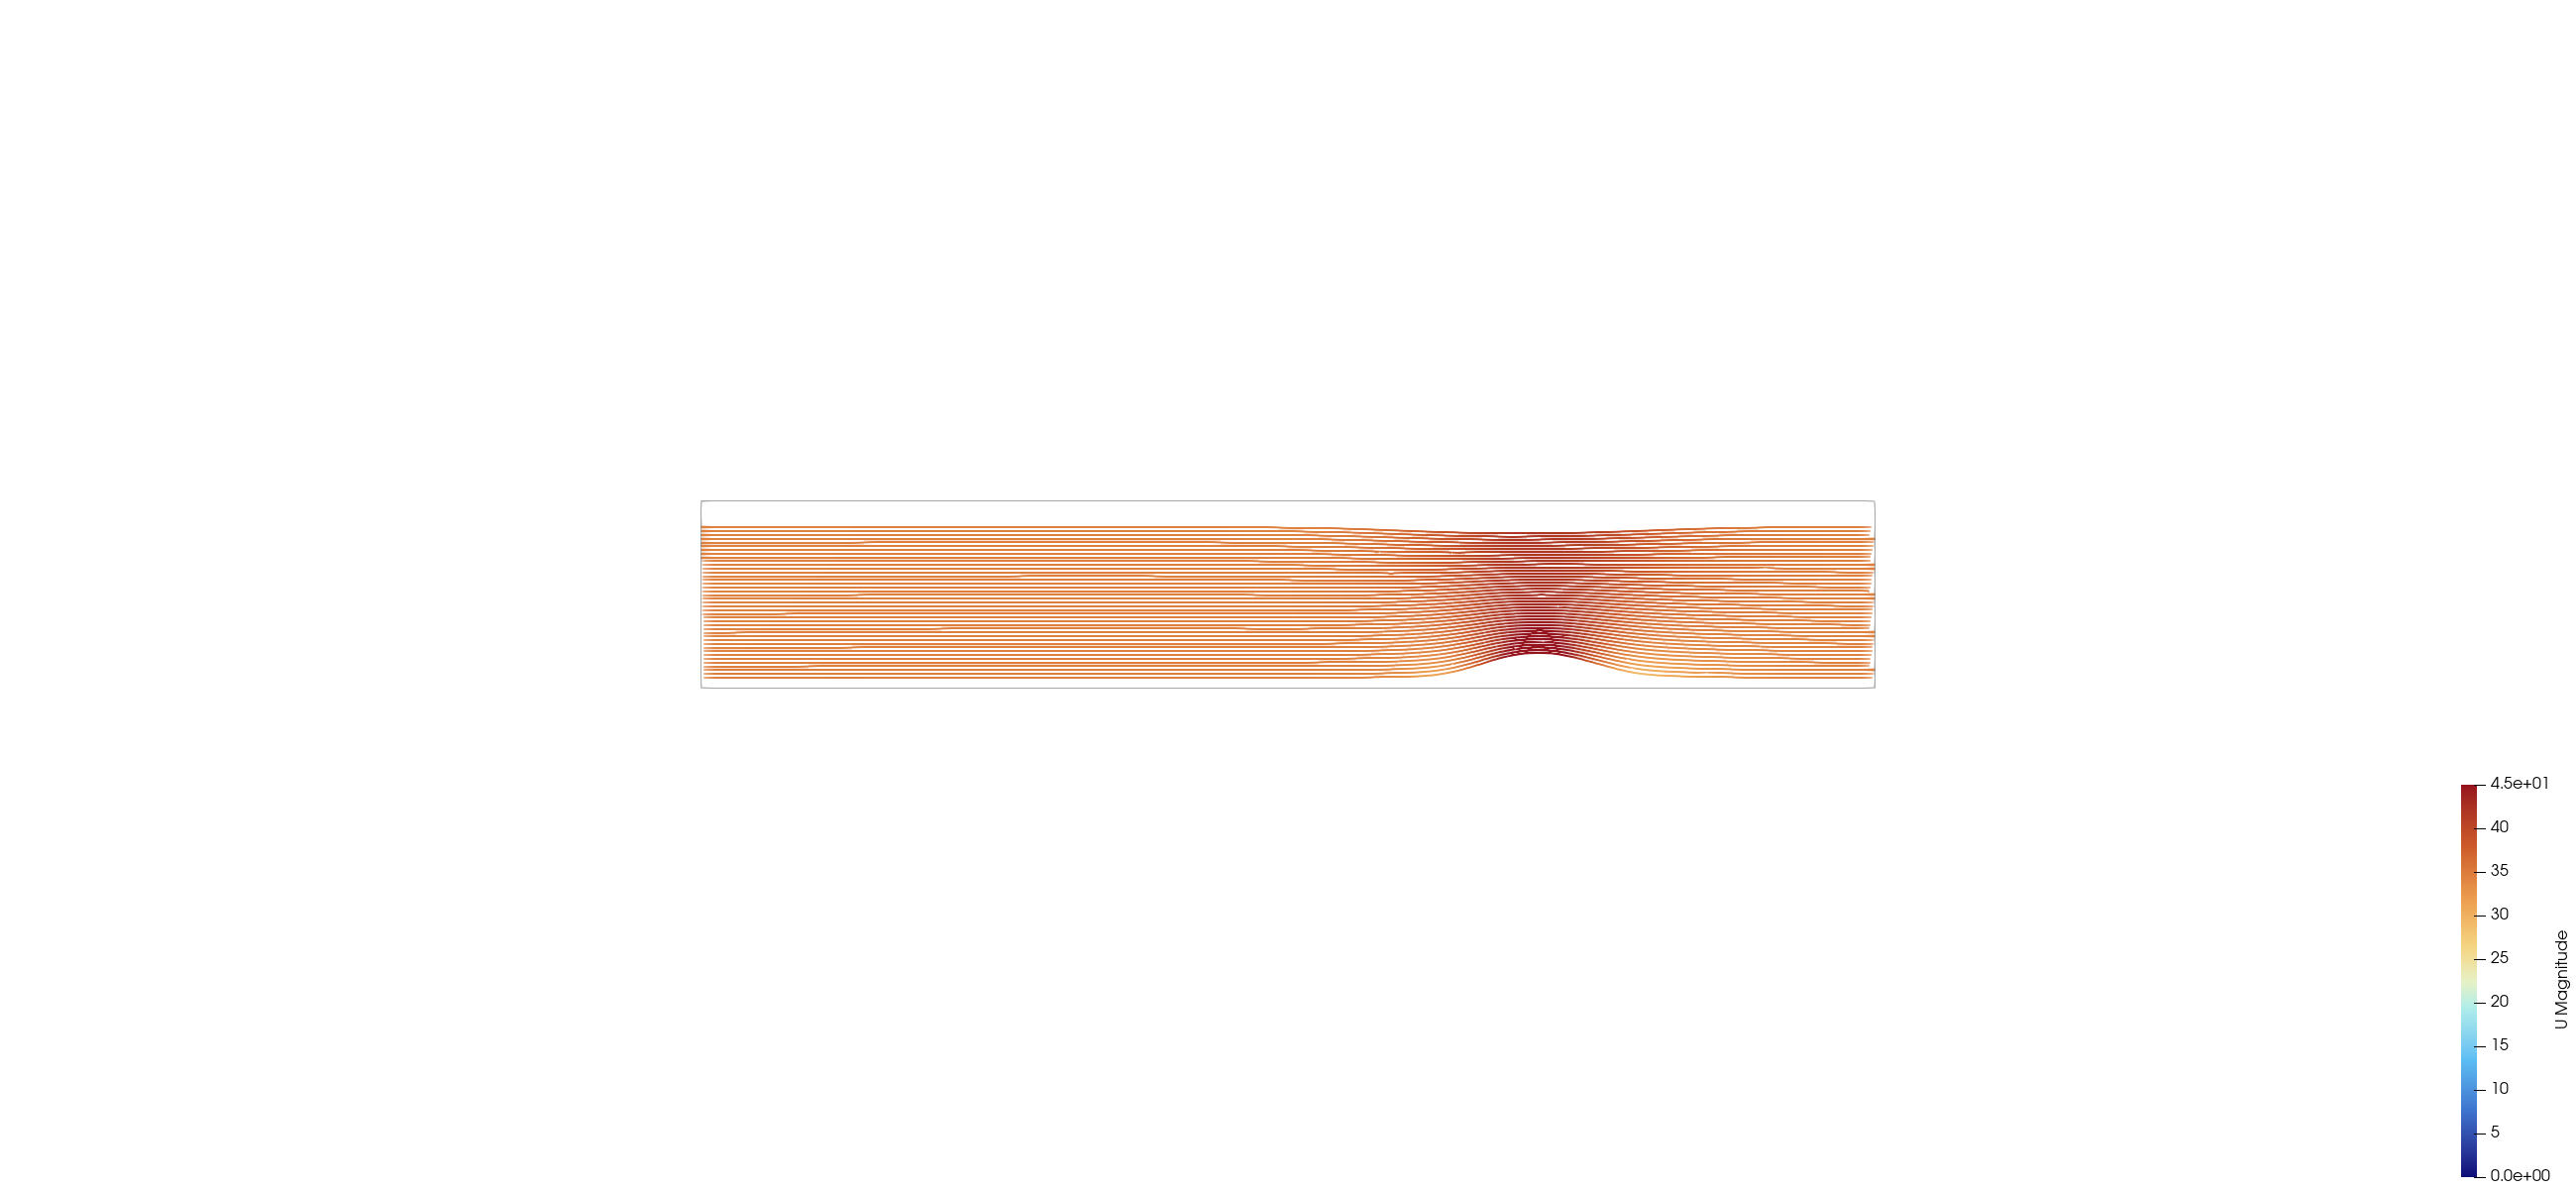
\includegraphics[width=0.90\linewidth]{figures_third_pass/paraview_streamlines.png}
\caption{Third-pass ParaView streamline-style rendering from the \texttt{.foam} case.}
\end{figure}

\begin{figure}[H]
\centering

\includegraphics[width=0.90\linewidth]{figures_third_pass/paraview_wall_shear.png}
\caption{Third-pass ParaView wall-focused rendering from the \texttt{.foam} case.}
\end{figure}

\section{Reproducibility}
From the repository root, the third-pass workflow is:
\begin{lstlisting}
NASA_HUMP_ONLY_TAGS=exp_uniform_sst_500 bash scripts/run_nasa_hump_improvement_sweep.sh
python3 scripts/evaluate_nasa_hump_second_pass.py
bash scripts/make_figures.sh
bash scripts/render_nasa_hump_paraview.sh
bash scripts/build_report.sh
\end{lstlisting}

To rerun the broader negative-result sweep for audit purposes:
\begin{lstlisting}
bash scripts/run_nasa_hump_improvement_sweep.sh
\end{lstlisting}

\section{Conclusion}
The third pass produced a genuine improvement, but not in the way the failed variants initially suggested. The winning change was not a more elaborate inlet, a more aggressive blockage contour, a denser mesh, or a different closure. The winning change was simply to trust the already-best second-pass SST configuration and run it farther, until the benchmark score itself stopped lagging behind the residual trend.

That outcome is useful because it is conservative, reproducible, and easy to defend. It improves the local MAE from \texttt{0.2038187409} to \texttt{0.1801372055} without introducing new unverified geometry or forcing the solution toward a hidden target. It also gives a clearer direction for any future pass: continue using experiment tables and benchmark scoring to reject seductive but non-improving changes, and only add new modeling complexity when it beats the simpler converged baseline honestly.

\bibliographystyle{plain}
\bibliography{references}

\end{document}
